\message{ !name(main.tex)}%pdflatex -shell-escape main.tex  
\documentclass[aspectratio=1610]{beamer}

\hypersetup{
        unicode=true,
        linkcolor=blue,
        anchorcolor=blue,
        citecolor=green,
        filecolor=black,
        urlcolor=blue
    }

%%%%% PACKAGES HERE
%% \usepackage{}
\usepackage{amsmath}
\usepackage{amssymb}
\usepackage{listings}
\usepackage[cache=false]{minted}
\usepackage{textcomp}
\usepackage{xcolor}

\usepackage[style=authortitle,backend=biber]{biblatex}
\addbibresource{references.bib}

%%%%%%%%%%%%%%%%%%%%%%%%%%%%%%%%%%%
%% DO NOT CHANGE

\usetheme{default}
\useinnertheme{circles}
\useoutertheme{infolines}
\usefonttheme{serif}

\usepackage{etoolbox}

%% T for navigation symbols
%%\setbeamertemplate{navigation symbols}{}

%% T for header
%% \setbeamertemplate{headline}{%
%%   \leavevmode%
%%   \ifdefempty{\insertsubsectionhead}{
%%     \begin{beamercolorbox}[wd=0.99\paperwidth,ht=2.25ex,dp=1ex,center]{section in head/foot}%
%%       % \hbox to .5\paperwidth{\hfil\insertsectionhead\hfil}
%%       \insertsectionhead
%%     \end{beamercolorbox}%
%%   }{
%%     \begin{beamercolorbox}[wd=.44\paperwidth,ht=2.25ex,dp=1ex,right]{section in head/foot}%
%%       % \hbox to .5\paperwidth{\hfil\insertsectionhead\hfil}
%%       \insertsectionhead
%%     \end{beamercolorbox}%
%%     \begin{beamercolorbox}[wd=.1\paperwidth,ht=2.25ex,dp=1ex,center]{section in head/foot}%
%%       % \hbox to .5\paperwidth{\hfil\insertsectionhead\hfil}
%%       -
%%     \end{beamercolorbox}%
%%     \begin{beamercolorbox}[wd=.44\paperwidth,ht=2.25ex,dp=1ex,left]{subsection in head/foot}%
%%       % \hbox to .5\paperwidth{\hfil\insertsubsectionhead\hfil}
%%       \insertsubsectionhead
%%     \end{beamercolorbox}
%%   }%
%% }

%% T for frame title
% \setbeamertemplate{frametitle}{%
%   \usebeamerfont{frametitle}\insertframetitle\strut%
%   \vskip-0\baselineskip%
%   \leaders\vrule width .95\paperwidth\vskip1pt%
%   \vskip0pt%
%   \nointerlineskip
% }

%% T for footer
% \setbeamercolor{footlinecolor}{fg=cyan,bg=green}
% \setbeamercolor{author in head/foot}{fg=blue}

\setbeamertemplate{footline}{%
  \leavevmode%
  \hbox{%
  % \begin{beamercolorbox}[wd=.26\paperwidth,ht=2.25ex,dp=1ex,left]{author in head/foot}%
  %   \hspace*{2ex}\usebeamerfont{author in head/foot} INFOTEC CDMX
  % \end{beamercolorbox}%

  % \begin{beamercolorbox}[wd=.50\paperwidth,ht=2.25ex,dp=1ex,center]{author in head/foot}%
  %   \usebeamerfont{title in head/foot} Aproximaci\'on de Campos Vectoriales con AP 
  % \end{beamercolorbox}%
  % \begin{beamercolorbox}[wd=.24\paperwidth,ht=2.25ex,dp=1ex,right]{date in head/foot}%
  %   \usebeamerfont{date in head/foot}
  %   \insertshortdate{}\hspace*{1em}  % date
  %   \insertframenumber/\inserttotalframenumber\hspace*{2ex}
  % \end{beamercolorbox}
}%
  \vskip0pt%
}
%%%%%%%%%%%%%%%%%%%%%%%%%%%%%%%%%%%%%%%%%%%%%%%%

%% Start from here.
\title{{\huge Aproximación de Campos Vectoriales con AP}}
\author{ \textbf{Daniel A. Cervantes Cabrera}\footfullcite{INFOTEC-CDMX},
        Miguel A. Moreles Vázquez\footfullcite{CIMAT-GTO} \\ ENOAN 2022 }
\date{7 de Julio, 2022}

\begin{document}

\message{ !name(main.tex) !offset(-3) }


\begin{frame}[plain]
  \titlepage
\end{frame}


\begin{frame}{Contenido}
  \tableofcontents

  % // This frame is the outline page which contains the full outline.
  \end{frame}


%   \begin{frame}
%   \tableofcontents[currentsection, subsectionstyle=show/show/hide]


% \end{frame}

\section{Introduction al AP}

\begin{frame}
  \frametitle{Un problema de clasificaci\'on}
\textit{  Deep Learning: An Introduction for Applied Mathematicians, Catherine F. Higham.}
  \begin{figure}[h]
    \centering
    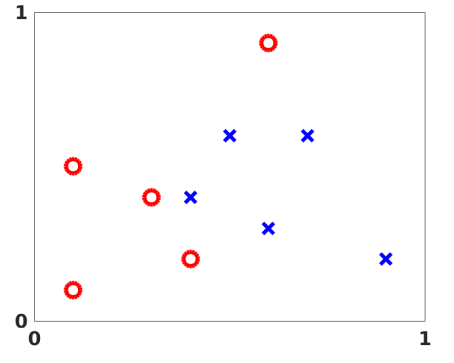
\includegraphics[scale=0.25]{fig}
    \caption{C\'irculos categoria A, Cruces categoria B. }
  \end{figure}
  
  Construir una función $F(\mathbf{x}):(0,1)\times (0,1)\to \mathbb{R}^2$ tal que,
  
  \begin{displaymath}
    F(\mathbf{x}) =
    \begin{cases}
      A = (1,0)^T \\
      B = (0,1)^T
    \end{cases}  
  \end{displaymath}
  
\end{frame}

\begin{frame}
  \frametitle{Redes Neuronales Computacionales}
  Aprendizaje Profundo (\textit{Deep Learning}): $F(x)$ es una \textquotedblleft Red Neuronal Computacional\textquotedblright.

  \begin{figure}[h]
    \centering
    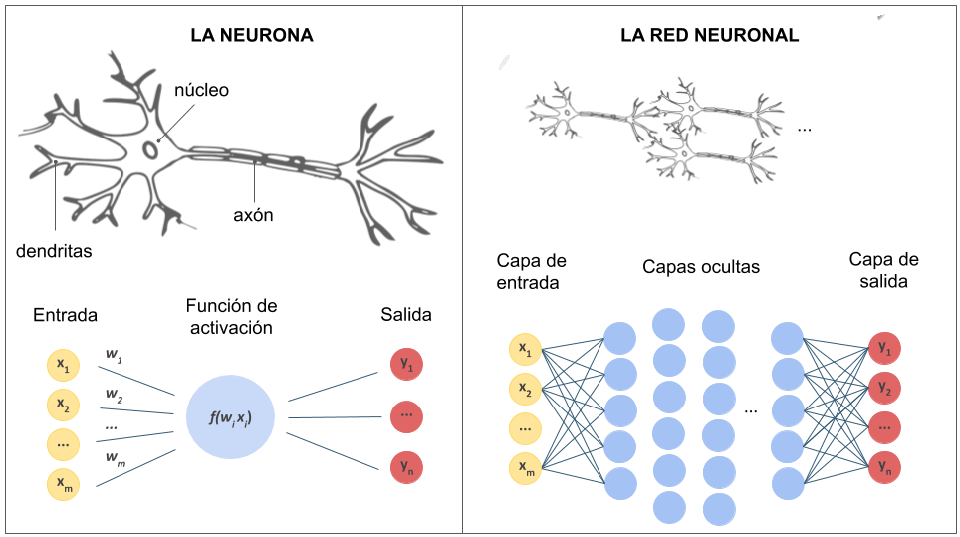
\includegraphics[scale=0.3]{fig2}
    \caption{Modelo simplificado de Red Neuronal Computacional. }
  \end{figure}

\end{frame}


% \begin{frame}
%   \frametitle{Funci\'on de activiaci'on}
%   Acci\'on en el n\'ucleo: funci\'on de activaci\'on.

  
%   E.g. Sigmoide:
%   \begin{align*}
%     \sigma(x) &= \frac{1}{1+e^{-x}} \\
%     \sigma(x)^\prime(x) &= \sigma(x)(1-\sigma(x))
%   \end{align*}

 
%   \begin{figure}[h]
%     \centering
%     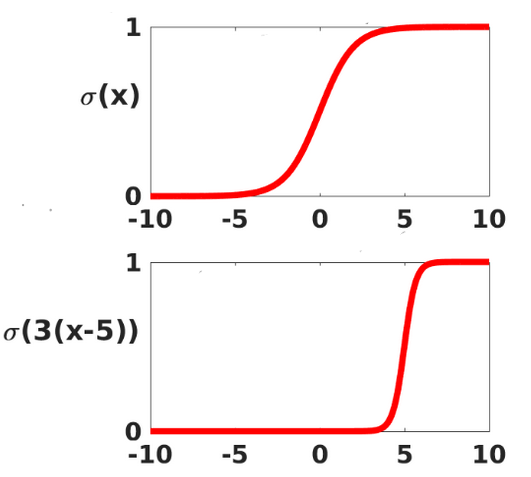
\includegraphics[scale=0.3]{fig3}
%     \caption{Funci\'on de activiaci\'on sigmoide}
%   \end{figure}

%  \end{frame}

\begin{frame}
  \frametitle{Funci\'on de Activaci\'on}
  Acci\'on sobre el n\'ucleo.
   \begin{columns}
     \begin{column}{0.3\textwidth}
       Para $z\in \mathbb{R}^m \; \sigma: \mathbb{R}^m\to \mathbb{R}^m$,
       \begin{displaymath}
         (\sigma(z))_i = \sigma(z_i).
       \end{displaymath}

       E.g. Sigmoide:
         \begin{align*}
           \sigma(x) &= \frac{1}{1+e^{-x}} \\
           \sigma(x)^\prime(x) &= \sigma(x)(1-\sigma(x))
         \end{align*}
         
     \end{column}

     \begin{column}{0.6\textwidth}  %%<--- here
       \begin{center}
         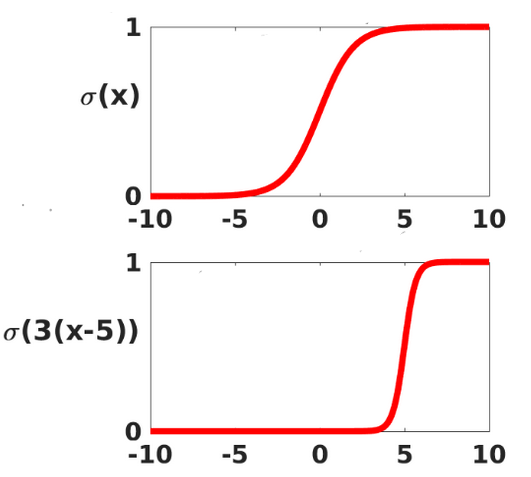
\includegraphics[width=8cm,height=6cm]{fig3}       
       \end{center}
     \end{column}
     %\caption{Funci\'on de activiaci\'on sigmoide}
   \end{columns}
 \end{frame}


 \begin{frame}{Ejemplo}
    \begin{columns}
    \column{0.4\textwidth}
       \begin{displaymath}
     x =
     \begin{pmatrix}
       x_1 \\
       x_2
     \end{pmatrix}
   \end{displaymath}
    \begin{displaymath}
      W^{[2]} =
      \begin{pmatrix}
        w_{11}^2 & w_{21}^2 \\
        w_{21}^2 & w_{22}^2 \\
      \end{pmatrix} \; b^{[2]} =
      \begin{pmatrix}
        b_1^2 \\
        b_2^2
      \end{pmatrix}
    \end{displaymath}

    \begin{displaymath}
      \sigma(W^{[2]}x+b^{[2]}) \in \mathbb{R}^2.
    \end{displaymath}

    \vspace{.5cm}
    \begin{displaymath}
      F(x) = \sigma(W^{[4]}(\sigma(W^{[3]}\sigma(W^{[2]}x+b^{[2]})+b^{[3]})+b^{[4]}) \in \mathbb{R}^2.
    \end{displaymath}
    \column{0.6\textwidth}
        \begin{figure}
        \centering
        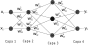
\includegraphics[width=8cm,height=5cm]{fig5}
        \caption{Red Neuronal de cuatro capas. }
        \end{figure}
    \end{columns}
\end{frame}



\begin{frame}
  \frametitle{Entrenamiento}
  \begin{itemize}
  \item  Por determinar:  $W := (W^{[1]},W^{[2]},W^{[3]},W^{[4]})$, $b:=(b^{[1]},b^{[2]},b^{[3]},b^{[4]})$ y $F(x,W,b)$.
  \item Datos de entrenamiento: $\{x_i\}_{i=1}^N$ y $\{y(x_i)\}_{i=1}^N$ donde
 \begin{displaymath}
      y(x) =
      \begin{cases}
        (1,0)^T & \textnormal{ si } x \textnormal{ es }  \color{blue} x  \\
        (0,1)^T &  \textnormal{ si }  x \textnormal{ es }  \color{red} o
      \end{cases}
    \end{displaymath}
  \item Funcional de costo:
    \begin{displaymath}
      L(W,b):=   \frac{1}{N} \sum_{i=1}^N \frac{1}{2} \|F(x_i,W,b) - y(x_i) \|_2^2
    \end{displaymath}
  \end{itemize}

  Objetivo: $L(W,b)\to 0$
    
  \end{frame}

  \begin{frame}
    \frametitle{Entrenamiento}

    \begin{itemize}
    \item   Supongamos que $W$ y $b$ se escriben en un vector $p$ tal que $p\in \mathbb{R}^s$ as\'i:
      \begin{displaymath}
        L: \mathbb{R}^s\to \mathbb{R}
      \end{displaymath}
    \item Método de optimizaci\'on:  \textquotedblleft Gradiente Descendiente \textquotedblright.
      %\pause
    \item Si $p=(p_1,\ldots,p_s)$ y $\Delta p = (\Delta p_1, \ldots, \Delta p_s)$. Entonces
      \begin{displaymath}
        L(p+\Delta p) \approx L(p) + \sum_{r=1}^{s} \frac{\partial L(p)}{\partial p_r} \Delta p_r = L(p) + \nabla L(p)^T \cdot \Delta p
      \end{displaymath}
    \item Por lo tanto,  $\Delta p = - \nabla L(p)$ \\
    \item $p \to p - \eta \nabla L(p)$. En donde  $\eta$, es la raz\'on de aprendizaje.
   
    \end{itemize}
  \end{frame}



  \begin{frame}
    \frametitle{Entrenamiento}

    \begin{itemize}
    \item Definiendo,
      \begin{displaymath}
        L_{x_i}(W,b) = \frac{1}{2} \|F(x_i,W,b) - y(x_i) \|^2_2
      \end{displaymath}
      entonces
      \begin{displaymath}
        \nabla L(W,b) = \frac{1}{N} \sum_{i=1}^N \nabla L_{x_i}(W,b).
      \end{displaymath}
      
    \item \textquotedblleft Gradiente Descendiente Estoc\'astico\textquotedblright:  $i\in random\{1,\ldots,N\}$.
      \begin{displaymath}
        p \to p - \eta \nabla L_{x_i}(W,b)
      \end{displaymath}
    \item Retropropagaci\'on. Para $2 \leq l \leq L$
      \begin{displaymath}
        \frac{\partial L}{\partial b_j^{[l]}} = \delta_j^{[l]}, \; \frac{\partial L}{\partial w_{jk}^{[l]}} = \delta_j^{[l]} \sigma_k(z^{[l-1]}); 
      \end{displaymath}
con
\begin{align*}
  \delta^{[L]} &= \sigma^\prime (z^{[L]})\cdot (\sigma(z^{[L]}) -y ) \\
  \delta^{[l]} &= \sigma^\prime (z^{[l]})\cdot (W^{[l+1]})^T\delta^{[l+1]}  \; \textnormal{para } 2\leq l\leq L-1\\
 \textnormal{con } z^{[l]}&=W^{[l]}\sigma(z^{[l-1]})+b^{[l]}\in \mathbb{R}^n_l  \textnormal{ para } l=2,\ldots,L.
\end{align*}

\end{itemize}
    
    %\begin{itemize}
    %   % \item 
    %   %     %   \begin{displaymath}
    %   %     %     L_{x_i} = \frac{1}{2} \|F(x_i,W,b) - y(x_i) \|^2_2 \; \nabla L(p) =  
    %   %     %   \end{displaymath}
    %   % \item \nabla 
    %   %     % \item 
    % \end{itemize}    

\end{frame}

\begin{frame}
  \frametitle{Predicci\'on}

  \begin{figure}[h]
    \centering
    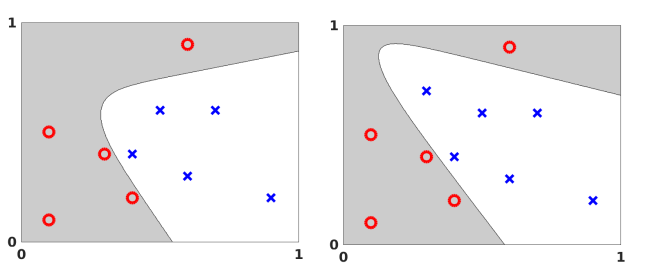
\includegraphics[scale=2]{fig7}
    \caption{Clasificaci\'on dados los conjuntos de entrenamiento. }
  \end{figure}
  
\end{frame}


  \section{Solución num\'erica de EDP con AP }
\begin{frame}
  \frametitle{ Soluci\'on  num\'erica de EDP }
  \textit{Sirignano and Spiliopoulos (2018)}
  
  Sea $u$ una funci\'on inc\'ognita definida en $\Omega \times [0,T]$ con $\Omega\in \mathbb{R}^d$ la cual satisface la siguiente EDP
  \begin{align*}
    \begin{cases}
      (\partial_t + \mathcal{L}) u(x,t)  &= 0  \qquad  (x,t)\in \Omega \times [0,T] \\
      u(x,0) & = u_0(x) \qquad x\in \Omega \\
      u(x,t) & = g(x,t) \qquad (x,t) \in  \Omega \times [0,T] 
    \end{cases}
  \end{align*}

  Objetivo: Aproximar $u$ con $F(x,t,W,b)$.

\end{frame}


\begin{frame}
  \frametitle{ Soluci\'on  num\'erica de EDP }
  \begin{itemize}
  \item  Una medida de qué tan buena es la  aproximación del operador diferencial:
  \begin{displaymath}
    a: = \| (\partial_t + \mathcal{L}) F(x,t,W,b) \|^2_{\Omega\times [0,T]}
  \end{displaymath}
  
\item Para la condición de frontera:
  \begin{displaymath}
    b:=\| F(x,t,W,b) - g({x},t)\|^2_{\partial \Omega \times [0,T]}
  \end{displaymath}
\item Para la condición inicial:
  \begin{displaymath}
   c:= \| F(x,0,W,b) - u_0(x)\|_{\Omega}
   \end{displaymath}
\end{itemize}
para una norma $L^2$. De donde podemos definir el funcional de costo 
\begin{displaymath}
  L(W,b) = a + b + c 
\end{displaymath}
\end{frame}

\begin{frame}
  \frametitle{ Algoritmo }
  \begin{enumerate}
  \item Inicializar los par\'ametros $W,b$ y la raz\'on de aprendizaje $\eta$.
  \item
    \begin{itemize}
    \item Generar $ni=\{(x^n_i,t^n_i)\}_{i=0}^{N_{inner}}$ en $\Omega\times [0,T]$
    \item Generar $nbdy=\{(z_i^n,\tau_i^n\}_{i=0}^{N_{bdy}}$ en $\Omega\times [0,T]$
    \item Generar $w=\{w_i^n\}_{i=0}^{N_{init}}$ en $\Omega$
    \end{itemize}
  \item Calcuar el funcional de costo $(x^n,t^n) = \{ ni,nbdy,w\}$
    \begin{displaymath}
      L(x^n,t^n,W^n,b^n) = a + b + c
    \end{displaymath}
  \item Actualizar los par\'ametros:
    \begin{align*}
      W^{n+1}  &= W^n - \alpha_n \nabla_{W^n} L(x_n,t_n,W_n,b_n) \\
      b^{n+1}  &= b^n - \alpha_n \nabla_{b^n} L(x_n,t_n,W_n,b_n)
    \end{align*}
  \item Repetir los pasos 2-4 hasta que los siguientes valores sean peque\~nos
    \begin{displaymath}
      \|W^{n+1} - W^n\| \; \|b^{n+1} - b^n\|
    \end{displaymath}

  \end{enumerate}
\end{frame}


\begin{frame}
  \frametitle{ Teorema Sirignano and Spiliopoulos (2018)}
  \begin{itemize}
  \item Si $L(W,b)$ el funcional de costo que mide la aproximaci\'on de una red neuronal  de operador diferencial, de frontera y condiciones inciales de una EDP.
  \item Sea $\mathcal{C}^n$ la clase de redes neuronales con $n$ capas ocultas.
  \item Si $f^n = \arg \min L(W,b)$. 
  \end{itemize}
Entonces
\begin{displaymath}
  f^n \to u \textnormal{ cuando } n \to \infty
\end{displaymath}

\end{frame}

\section{Aproximaci\'on de campos vectoriales }
\begin{frame}{Aproximaci\'on de campos vectoriales }
 
  \begin{itemize}
  \item Dinámica de fluidos computacional.
  \item Aplicaciones en Meteorología.
    \begin{itemize}
    \item Aproximaci\'on de velocidades de viento considerando condiciones f\'isicas.    
    \item Dispersi\'on de contaminantes.
    \item Modelos de predicci\'on de concentraciones de contaminantes de aire.  
    \end{itemize}
  \end{itemize}

\end{frame}



\begin{frame}{Formulaci\'on }
  \begin{itemize}
  \item   Sea $\mathbf{U}_{obs}^0 = \{ (u_{1,i}(\mathbf{x}_i),(u_{2,i}(\mathbf{x}_i) \}_{i=1}^N$ un campo vectorial sobre una región acotada $\Omega\subset \mathbb{R}^3$ que representa un conjunto de observaciones de velocidades de viento. 
  \item Se requiere construir una funci'on $u(\mathbf{x})$
  \end{itemize}

\end{frame}




% \subsection {Esquemas variacionales}
% \begin{frame}
%   \frametitle{Frame Title 1}
%   Example Example
% \end{frame}


\section {Caso de estudio}
\begin{frame}{Frame Title 2}
  Example Example

\begin{itemize}
    \item item 1
    \item item 2
\end{itemize}

\end{frame}




\end{document}
\message{ !name(main.tex) !offset(-412) }
